\documentclass[a4paper,12pt]{article}
\usepackage[margin=2cm]{geometry}
\usepackage{fancyhdr}
\usepackage[utf8]{inputenc}
\usepackage[czech]{babel}
\usepackage{float}
\usepackage{graphicx}

\setlength{\headheight}{15pt}
\pagestyle{fancy}
\fancyhf{}
\fancyhead[L]{07\_rec-rep}
\fancyhead[R]{Pavel Pernička}
\fancyfoot[C]{\thepage}
\renewcommand{\headrulewidth}{0.4pt}

\begin{document}

\section*{Výběr klasifikátoru}
\renewcommand{\thesubsection}{\arabic{subsection}.}

\subsection{Výběr vhodného parametru}
Než začneme vůbec hledat nejlepší parametr pro klasifikátor $C_1$, podíváme se, jaké situace obsahuje soubor s ground-truth. Vídíme, že počet pozitivních a~negativních situací je dostatečně velký (50) a zároveň se počty shodují. Máme tedy relevantní situace k tomu, aby mělo smysl hledat samotný parametr. 

Abychom mohli dále pokračovat, pro jednotlivé parametry $\alpha$ spočítáme množství $TP$, $TN$, $FN$, $TN$ případů ze srovnání ground-truth a výsledků klasifikátoru $C_1$. Z těchto tříd vypočítáme recall ($TPR$) a $FPR$, které vykreslíme do obrázku \ref{fig:roc_curve}. Když spojíme takto vzniklé body ve všech dostupných hodnotách $\alpha$, získáváme ROC křivku. 

Bod obecně nejlepšího $\alpha$ hledáme jako bod nejblíže (ve smyslu eukleidovské vzdálenosti) k bodu $(0,1)$, kde by byl klasifikátor optimální, tedy že by určil všechny pozitivní případy správně a zároveň by nikdy neklasifikoval jako pozitivní to, co pozitivní není. Zde jsme našli $3$~nejbližší body na stejných souřadnicích, a~to $\alpha = \alpha_{22}$, $\alpha = \alpha_{23}$, $\alpha = \alpha_{24}$.

\begin{figure}[H]
    \centering
    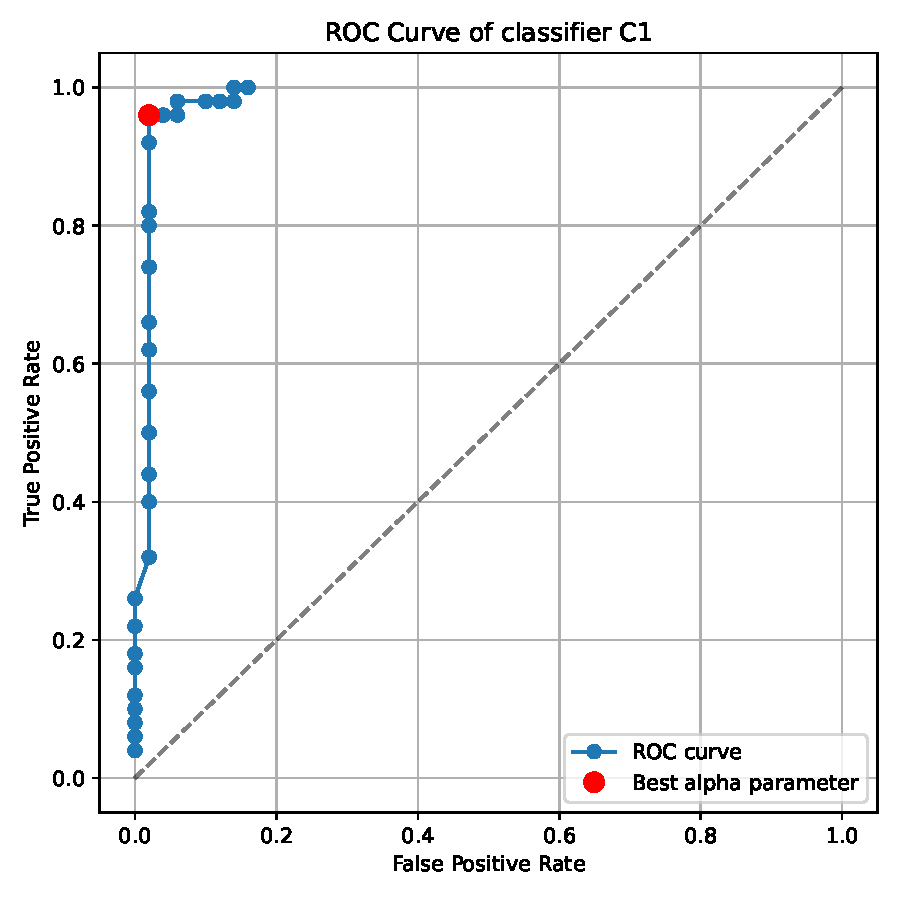
\includegraphics[width=0.85\textwidth]{roc.pdf}
    \caption{ROC křivka klasifikátoru $C_1$}
    \label{fig:roc_curve}
\end{figure}

\subsection{Přísně tajné}
V této části máme díky dostatku času možnost opakovat načtení otisku prstu vícekrát. To nám mírně mění nároky na náš klasifikátor, protože nám to umožňuje minimalizovat $FPR$ částečně i~na úkor $TPR$, což omezí riziko neoprávněného přístupu k tajným dokumentům. Použijeme metriku, která bude uvnitř pravého $\epsilon$-okolí nulového $FPR$ hledat maximum rozdílu $TPR-FPR$. 

Při určování jsem vzhledem k citlivosti dat zvolil $\epsilon:= 0.01$, pro které mi vyšel nejlepší klasifikátor $C_4$ s $\alpha=\alpha_{11}$, kde $TPR=0.46$, což sice znamená nutnost přikládat prst ke čtečce několikrát, ale riziko průniku cizího uživatele je minimální. Na druhou stranu bude ale klasifikátor náchylný k malým změnám struktury otisku, takže např. agent s odřeným prstem bude mít výrazně nižší šanci dostat se do vlastního trezoru. 

Posuneme-li hranici na $\epsilon := 0.02$, což je stále přijatelná hodnota, bude metrice vyhovovat lépe klasifikátor $C_1$ s~$\alpha = \alpha_{22}$ a $TPR=0.94$, tentokrát s menším rizikem, že se agent nedostane do svého vlastního trezoru. Ale vzhledem k tomu, že je lepší variantou zabezpečená data zničit, než aby se k nim, byť s malou šancí dostal někdo jiný, raději zvolíme první variantu.

\begin{figure}[H]
    \centering
    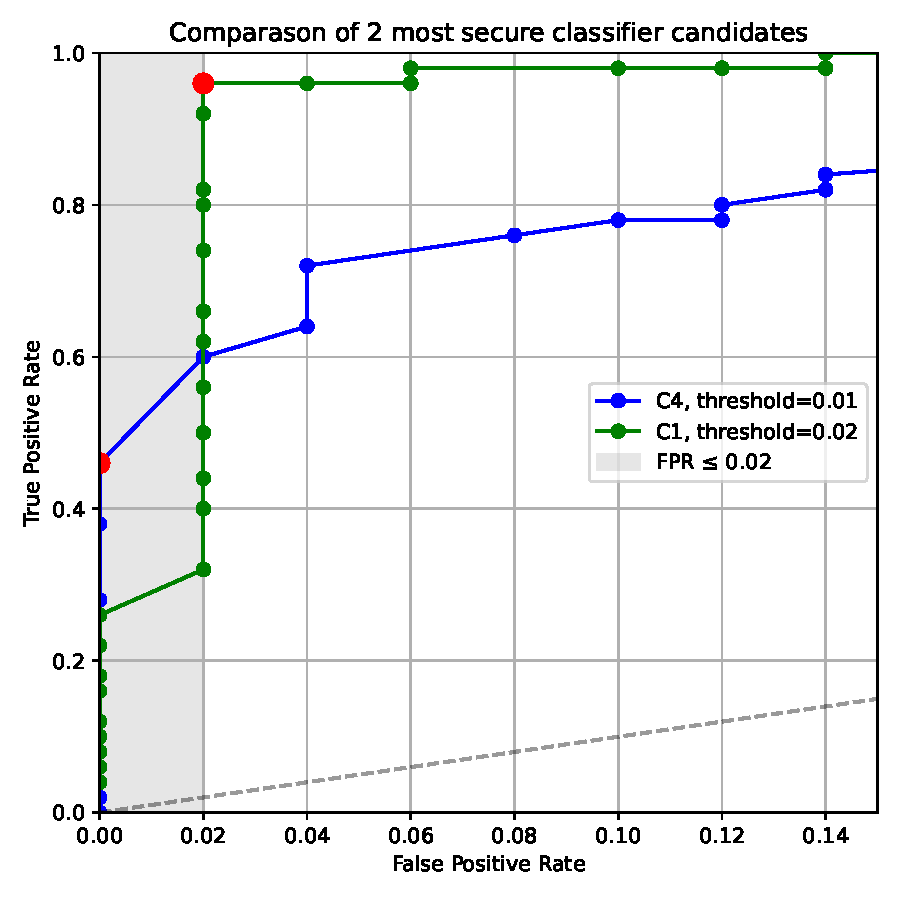
\includegraphics[width=0.8\textwidth]{roc_comparison.pdf}
    \caption{Porovnání ROC křivek klasifikátorů $C_1$ a $C_4$}
    \label{fig:roc_comp}
\end{figure}

\subsection{Hlavně bezpečně}
Pro určení, jestli je cizí klasifikátor lepší než náš nejlepší, použijeme metriku popsanou v~předchozím úkolu. V přiloženém souboru se jedná o funkci \textit{is\_better()}.
\end{document}
